\documentclass[a4paper]{scrreprt}
\usepackage{fancyhdr}
\pagestyle{fancy}
\usepackage[english]{babel}
\usepackage[utf8]{inputenc}
\usepackage{graphicx}
\usepackage{url}
\usepackage{textcomp}
\usepackage{amsmath}
\usepackage{lastpage}
\usepackage{pgf}
\usepackage{wrapfig}
\usepackage{fancyvrb}
\usepackage{appendix}
\usepackage{pdfpages}
\usepackage{xcolor}
\usepackage{hyperref}

\hypersetup{
    colorlinks=true,
    linkcolor=blue,
    filecolor=black,      
    urlcolor=blue,
    citecolor=black,
}

% Create header and footer
\headheight 27pt
\pagestyle{fancyplain}
\lhead{\footnotesize{Datalagring, IV1351}}
\chead{\footnotesize{Seminar 1}}
\rhead{}
\lfoot{}
\cfoot{\thepage\ (\pageref{LastPage})}
\rfoot{}

% Create title page
\title{Seminar 1}
\subtitle{Datalagring, IV1351}
\author{Adrian Jonsson Sjödin \\ adriansj@kth.se}
\date{\today} 


\begin{document}

\maketitle

\tableofcontents %Generates the TOC

\chapter{Introduction}
The purpose of this seminar is to practice modeling information based on an organizational description that will later be turned into a functioning database. The first
step in this is to produce a conceptual model. The creation and reasoning behind this conceptual model is what will be covered in this report.

\chapter{Method}
To get our conceptual model we followed the same process as in IV1350 Object Oriented Design when we created our DM. We started
with noun identification, followed by using a category list (see \ref{fig:categoryList}) to try and get all the entities. After those two steps where done
we have quite a lot of entities, some of which where duplicates but with slightly different names. The next step now was
to go trough all of the entities and decide which we should keep and which where unnecessary, and then from there we started
grouping similar entities together and turn some of them to attributes. At the same time as we turned entities to attributes
and found new attributes we also specified the cardinality for them. Finally when we where satisfied with this we started to
draw associations between entities.

The software used to create the conceptual model is Astah Professional. This was chosen because I'm already familiar with it
from the previous mentioned course. One thing with it though is that it wasn't possible to specify 0..1 cardinality for the
associations. Thus all associations have the bubble indicating 0 on them.


\begin{figure}[h]
    \begin{center}
        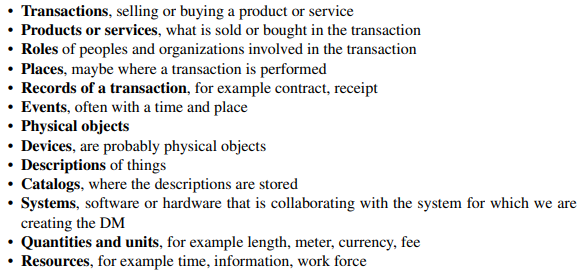
\includegraphics[width=.9\textwidth]{../img/CategoryList.PNG}
        \caption{Category list. \\ \textit{L Lindbäck, A First Course in Object Oriented Development, A Hands-On Approach, 2022}}
        \label{fig:categoryList}
    \end{center}
\end{figure}



\chapter{Result}
\label{sec:result}
In figure \ref{fig:nounCategoryList} we have the result from using noun identification and a category list.

\begin{figure}[h]
    \begin{center}
        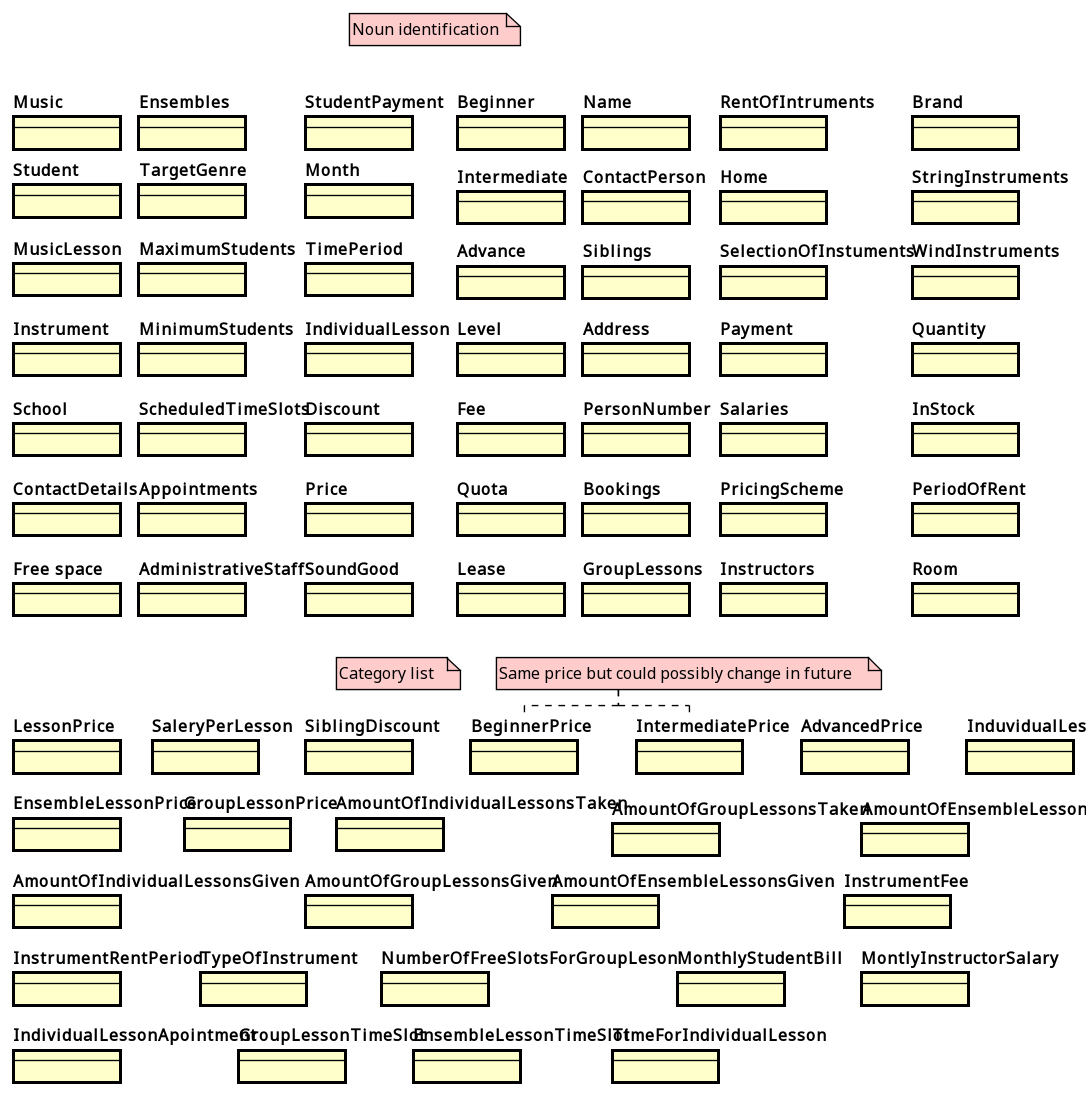
\includegraphics[width=.8\textwidth]{../img/noun-and-category.png}
        \caption{Found entities from noun identification and category list}
        \label{fig:nounCategoryList}
    \end{center}
\end{figure}

In figure \ref{fig:conceptualModel} we can see the finished conceptual model. I tried to have zero duplicated data and derived
data. That is why I have an entity called \textit{person} who contains all information that both a student and an instructor should have,
and had the \textit{student} and \textit{instructor} entity just contain relevant attributes unique to them. I also don't have
an attribute \textit{total} anywhere in the conceptual model since that would be derived data, and can for example in the
\textit{MonthlyStudentBill} be calculated from tha information in \textit{PricingScheme} and its own attributes.
\begin{figure}[h]
    \begin{center}
        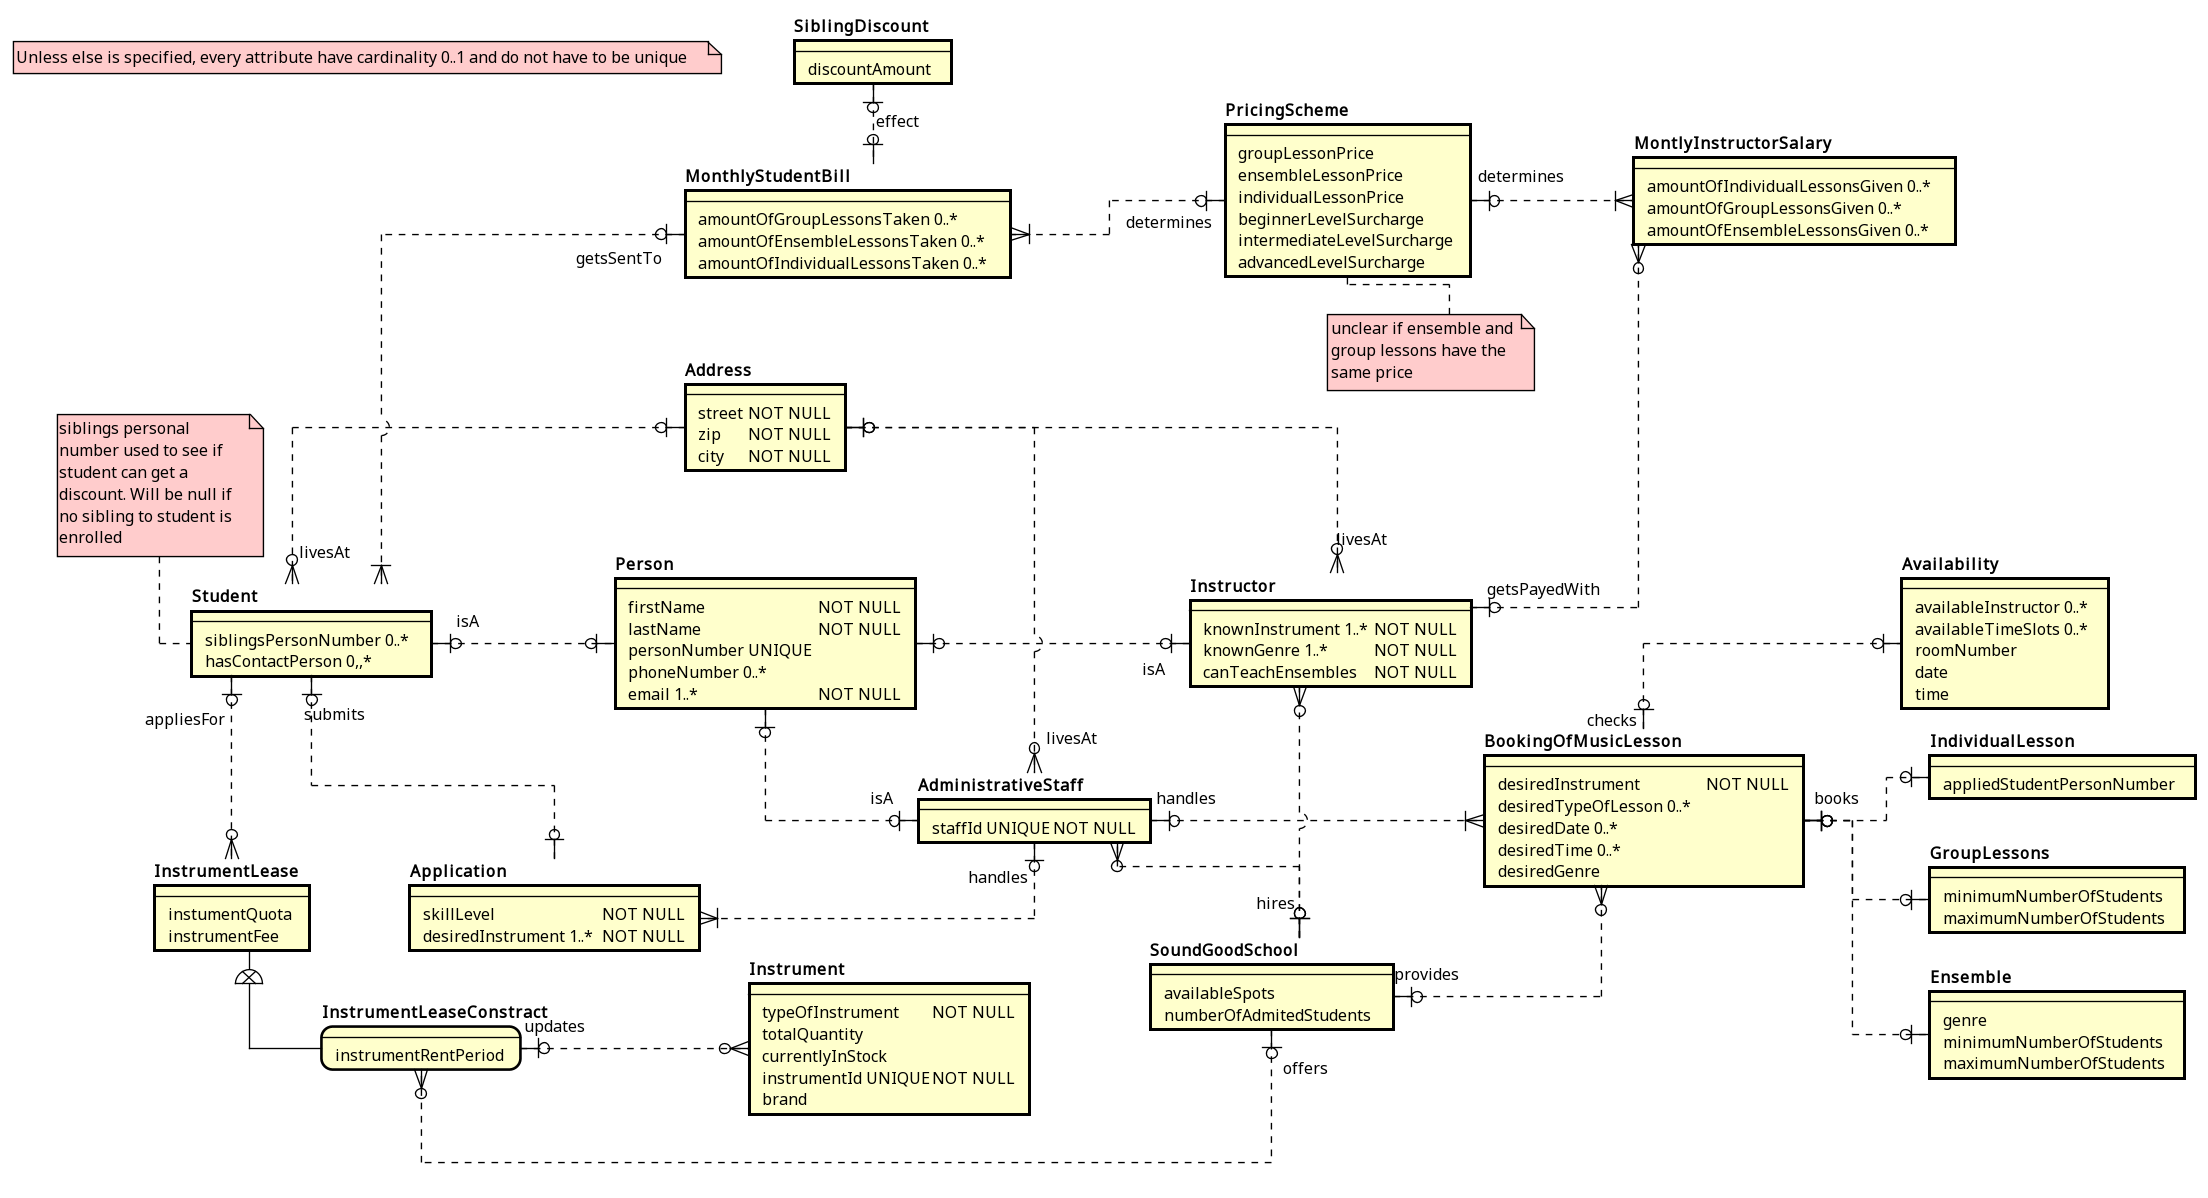
\includegraphics[width=\textwidth]{../img/conceptualModel.v1.0.1.png}
        \caption{Conceptual Model for the SoundGood music school database}
        \label{fig:conceptualModel}
    \end{center}
\end{figure}

\chapter{Discussion}
This is my first attempt at modeling a database but I think I've gotten everything that was specified in the customer description.
I have quite a few attributes that are not allowed to be nulled and for those I've simply decided that upon what I think the
customer would want since it wasn't specified if null values where allowed. For example in the entity \textit{Instructor}
all three attributes are not allowed to be null, this because it stands to reason that an employer would want to know which
instruments an instructor knows and what genres they can teach.

The customer description mentioned that there should be possible to store a contact person for a student, but not that they
must have one. Because of this I had an entity called \textit{ContactPerson} in an earlier version of my conceptual model, however]
since I strived to have no duplicated data I had to remove it since that entity then became empty. Instead we have an attribute
\textit{hasContactPerson} in \textit{Student} that will have a reference to \textit{Person} for the contact person. This is also
the reason why the attribute \textit{personNumber} can be null, since there is no point in storing the person number for a
contact person.

There is also an entity \textit{BookingOfMusicLesson} for which it can be argued that its associations might be a bit weird.
My thought behind it was that the administrative staff handles a booking by checking what the student wants and then look at
what is available and can offered to the student. That then books one out of the three lesson types. But reading the name now,
for example "\textit{BookingOfMusicLesson books IndividualLesson}" does come across a bit strange. Perhaps a better name might
have been just \textit{MusicLesson}.

Apart from the above mentioned I believe the conceptual model is sufficient and that it follows the rules and constraints that
a conceptual model should have. Naming conventions have been followed and every entity has an associations and every attribute
have its cardinality specified.

\end{document}
